%************************************************
\chapter{Connecting to a Cloud Service}\label{ch:introduction}
%************************************************

There are multiple ways of connecting to the different types of cloud services. They vary greatly depending on wich type you want to address. Since we only need to connect to a \ac{SaaS} based service, we will only discuss the possible connection alternatives for it.

A mobile application, like the Job Portal Aggregator, will live inside a device with almost uninterrupted access to the internet. This level of connectivity allows us to consider an abundance of protocols and methods for connecting any type of application to a cloud service.

The whole point of the cloud is to have an infrastructure that is always available and always connected, this means that the main point of entry to these kind of services is the internet, and by default the \ac{IP}. This means that we can use any type of transport protocol that builds upon the \ac{IP} Protocol to transmit information from and to a cloud service.\footnote{\url{http://en.wikipedia.org/wiki/IP_protocol}}  

Since the Job Portal Aggregator will be connecting to a \ac{SaaS} Application and, given the fact that the majority of \ac{SaaS} applications are web-based; which means they can be controlled via a web interface or via the HTTP Protocol \cite{mcwherter:2012}; we can consider the following two very different approaches for communicating with our cloud service: \textit{WebSockets} and \textit{RESTful APIs}

\section{RESTful APIs}
In his doctoral dissertation, \citeauthor{fielding:2000} generalized the Web's architectural principles and presented them as an architectural style. He described the interplay between resources, and the role of unique identifiers in such systems. He also talked about using a limited set of operations with strictly defined semantics to build a global infrastructure that can support any type of application. Fielding referred to this architectural style as \ac{REST}. \ac{REST} describes the Web as a distributed hypermedia application whose linked resources communicate by exchanging representations of resource state. \cite{webber:2010}

\begin{quotation}
In a hypermedia system, application states are communicated through representations of uniquely identifiable resources. The identifiers of the states to which the application can transition are embedded in the representation of the current state in the form of links.
\cite[p. 13]{webber:2010}
\end{quotation}

The term RESTful \ac{API} is given to an Application Programming Interface that is accessible via the HTTP Protocol and complies with the \ac{REST} architectural pattern.

One of the biggest advantages of a RESTful \ac{API} is that it allows you to perform different actions based on the state of the application, thus providing constraints on what the user of the application is allowed to do.

Communication with a RESTful service is done via HTTP and can be managed via its different verbs. This means that a single \ac{URI} can be used for different actions.

\begin{table}[H]
    \myfloatalign
  \begin{tabularx}{\textwidth}{Xll} \toprule
    \tableheadline{HTTP Verb} & \tableheadline{URI} & \tableheadline{Action}\\ 
    \midrule
    GET & /publications/1 & Show Publication with id: 1\\
    DELETE & /publications/1 & Delete Publication with id: 1\\
    PATCH & /publications/1 & Change Publication with id: 1\\
    GET & /publications & See all Publications\\
    POST & /publications & Create new Publication\\         
    \bottomrule
  \end{tabularx}
  \caption[HTTP Verbs and Actions]{HTTP Verbs and Actions} \label{tab:http_verb}
\end{table}

This approach works great with applications that don't need a constant stream of information coming from the server. It is reliable, easy to use and easy to configure. It even comes baked into one of the most popular frameworks for web development, Ruby on Rails.  



\section{Websockets}
WebSockets are part of the Connectivity section of the HTML5 specification. This section aims to help simplify some of the areas where browser limitations prevented developers from creating rich and immersive web application or where development was becoming overly complex. 
\cite[p. 7]{wang:2013} These areas include connectivity performance and real-time communications. 

A WebSocket is a full-duplex, bidirectional, single-socket connection, that allows a connection channel to remain open and, unlike normal HTTP connections, it lets you send information to the client through this channel without the need for the clients interaction, thus enabling real-time communication.

This type of communication drastically reduces latency, bandwidth and CPU power consumption and greatly simplifies the communication procedure and implementation. \cite{wang:2013} \autoref{fig:websocket} illustrates the differences in latency between simple polling and WebSockets.  

\begin{figure}[H]
    \begin{center}
        {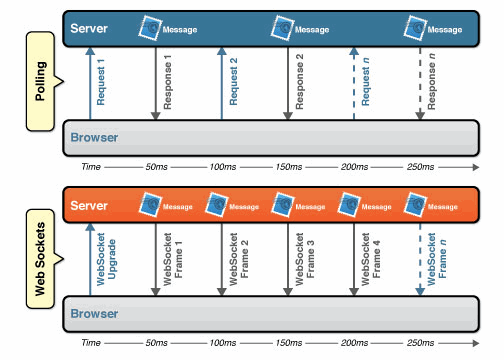
\includegraphics[width=1\linewidth]{gfx/websocket}}
        \caption[Polling vs. WebSocket]{Polling vs. WebSocket\footnotemark}\label{fig:websocket}
    \end{center}
\end{figure}
\footnotetext{Source: \url{http://www.websocket.org/img/latency-comparison.gif}}\\

Compared to a RESTful API, WebSockets are more difficult to implement, but that is of no importance, since they basically serve different purposes. WebSockets can't represent state, but are great for streaming data and real-time communications.

In the end it depends on the type of application to which you want to connect. A chat client or multiplayer game, for example, needs constant communication with the cloud service. An application like Twitter need information from the service often, but doesn't need an always open connection.

The Job Portal Aggregator works more like Twitter, than a multiplayer game, and doesn't need constant communication with the server, so our method for connecting to the MHM servers will be a RESTful \ac{API}.

\section{Transmitting Data through a RESTful API}
There are several ways of packaging and transmitting data from any kind of \ac{API} to a client. Most of these formats have been standardized and are compatible with a lot of programming languages.

Since we are talking about web services here, you could use the WebServices Standard. This standard defines several protocols and formats for transmitting and packaging data. These formats are based on the \ac{XML} and the most used is the \ac{SOAP}, a protocol specification for exchanging structured information. 

\ac{SOAP} consists of three parts: an envelope, which defines what is in the message and how to process it, a set of encoding rules for expressing instances of application-defined datatypes, and a convention for representing procedure calls and responses.\footnote{\url{http://en.wikipedia.org/wiki/SOAP}}

The big disadvantage of using \ac{SOAP} is that it suffers from a big overhead, because of the extra information it encompasses. Compared to vanilla \ac{XML}, \ac{SOAP} takes more space and can also cause overhead on the processing application, because of the increased complexity.

For the purposes of our application, a protocol like \ac{SOAP} is actually overkill. We don't need extra information about how to process the data, when we know how the data is serialized and structured. Rails supports \ac{XML} and \ac{JSON} formats for serialization of objects, so we will take a further look into how they look and behave.

\subsection{XML}
The goal of \ac{XML} is to define a set of rules for encoding documents in a format that is both human-readable and machine-readable. Although the design of XML focuses on documents, it is widely used for the representation of arbitrary data structures, for example in web services.\footnote{\url{http://en.wikipedia.org/wiki/Xml}}

\lstset{language=XML}
\begin{lstlisting}[frame=lt,caption=An XML example]
<?xml version="1.0" encoding="ISO-8859-1"?>
<CATALOG>
  <CD>
    <TITLE>Empire Burlesque</TITLE>
    <ARTIST>Bob Dylan</ARTIST>
    <COUNTRY>USA</COUNTRY>
    <COMPANY>Columbia</COMPANY>
    <PRICE>10.90</PRICE>
    <YEAR>1985</YEAR>
  </CD>
</CATALOG>

\end{lstlisting}

\subsection{JSON}

\ac{JSON} is an open standard format that uses human-readable text to transmit data objects consisting of attribute-value pairs. It is used primarily to transmit data from web applications, as an alternative to XML. Although originally derived from the JavaScript language, JSON is a language-independent data format that is compatible with a large variety of programming languages.\footnote{\url{http://en.wikipedia.org/wiki/JSON}}

%\lstset{language=json}
\begin{lstlisting}[frame=lt,caption=A JSON example]
{ 
  "catalog" : [{
      "title"  : "Empire Burlesque",
      "artist" : "Bob Dylan",
      "country": "USA",
      "company": "Columbia",
      "price"  : 10.90,
      "year"   : 1985
  }]
}
\end{lstlisting}

\subsection{Final Thoughts}

For the purpose of our use case, both formats are equivalent and offer us the same functionality. Depending on the type of data you want to transfer, deciding between the two can come down to which one is more compatible with your programming language of choice or which syntax you like the most. 

In the end, however, \ac{XML} has extra features that are not supported by \ac{JSON} and, thanks to its extensibility, can offer a greater degree of flexibility.

When communicating with our cloud service, we will use a mixture of \ac{JSON} and \ac{XML} depending on the action the mobile application wants to perform. 



   
  




 
  